\documentclass[aps,prl,reprint,superscriptaddress,nofootinbib,amsmath,amssymb]{revtex4-2}

\usepackage{graphicx}
\usepackage{dcolumn}
\usepackage{bm}
\usepackage{hyperref}
\usepackage{xcolor}

\begin{document}

\title{Resolving the Cosmological $H_0$ Discrepancy via Local Scalar-Tensor Scaling within the KBC Underdensity}

\author{Johannes Werner Schenk}
\email{info@johannes.schenk.com} 
\affiliation{Independent Researcher, Germany}

\date{\today}

\begin{abstract}
The persistent $5\sigma$ tension between the global Hubble constant ($H_0$) inferred from Planck cosmic microwave background (CMB) anisotropies and local distance ladder calibrations by the SH0ES collaboration represents a fundamental observational impasse. In this Letter, we present a localized, gauge-independent resolution operating within a generalized scalar-tensor framework formulated in the Jordan frame. Rather than introducing exotic early universe modifications, we model the local cosmic environment as a significant macroscopic underdensity ($\delta \approx -0.4$), consistent with empirical constraints on the Keenan-Barger-Cowie (KBC) super-void. By mapping the conformal scaling of the local metric tensor under a non-minimally coupled scalar field, the apparent local kinematic rate is shown to emerge naturally as a function of the environmental density profile. We demonstrate that a universal vacuum coupling parameter of $\beta \approx 0.157$ seamlessly aligns the background field equations with the local SH0ES metric horizon ($H_0 \approx 73.04 \text{ km s}^{-1}\text{Mpc}^{-1}$), rendering the tension an environmental boundary effect without altering pre-recombination physics.
\end{abstract}

\maketitle

\section{Introduction}
The concordance cosmological model ($\Lambda$CDM) demonstrates remarkable precision on ultra-large scales, yet it faces severe structural tensions when evaluated against local observational baselines \cite{Planck2018}. The discrepancy between the early-universe predictive horizon ($H_0 = 67.4 \pm 0.5 \text{ km s}^{-1}\text{Mpc}^{-1}$) and late-universe direct measurements ($H_0 = 73.04 \pm 1.04 \text{ km s}^{-1}\text{Mpc}^{-1}$) has resisted systematic corrections, strongly indicating an incomplete formulation of local gravitational interactions \cite{Riess2022}.

Conventional extensions trying to reconcile this gap typically inject new degrees of freedom prior to recombination, such as Early Dark Energy (EDE). These solutions, however, frequently induce secondary tensions in large-scale structure (LSS) growth parameters. 

In this work, we propose a parsimonious alternative: a localized, conformal modulation of the apparent kinematic scale driven by a scalar field coupling within the Jordan frame. This mechanism operates strictly within the geometric boundaries of the Keenan-Barger-Cowie (KBC) void, a massive local underdensity extending to approximately $300\text{ Mpc}$ with an empirically established density contrast of $\delta \approx -0.4 \pm 0.1$ \cite{Haslbauer2020}.

\section{Theoretical Framework}
We formalize the underlying dynamics within a ghost-free scalar-tensor architecture where the matter fields couple non-minimally to a conformal geometry. The total action of the theory in the Einstein frame is defined as:
{\small
\begin{equation}
S = \int d^4x \sqrt{-g} \left[ \frac{M_*^2}{2} R - \frac{1}{2}g^{\mu\nu}\partial_\mu\phi\partial_\nu\phi - V(\phi) \right] + S_m[\psi_m; \tilde{g}_{\mu\nu}]
\end{equation}
}
where $M_*$ represents the fundamental reduced Planck mass scale, $R$ is the Ricci scalar, and $V(\phi)$ denotes the self-interaction potential of the scalar field $\phi$. The matter fields $\psi_m$ reside in the physical Jordan frame, where the effective metric tensor $\tilde{g}_{\mu\nu}$ represents the frame of standard observers, related to the background geometry via the conformal mapping:
\begin{equation}
\tilde{g}_{\mu\nu} = A^2(\phi)g_{\mu\nu} = \exp \left( -\frac{2\beta\phi}{M_*} \right) g_{\mu\nu}
\end{equation}
where $\beta$ denotes the dimensionless, universal coupling constant of the vacuum architecture. Crucially, Eq. (1) belongs to the general Horndeski class, where the specific choice of $V(\phi)$ triggers a non-linear chameleon screening mechanism in high-density environments, effectively restoring General Relativity within deep stellar interiors and screening standard candles.

When evaluating the field equations derived from Eq. (1), local matter density gradients act as direct source terms for the spatial configuration of the field. In the quasi-static limit, assuming a flat effective potential field response ($V_{,\phi} \approx 0$), the Klein-Gordon equation simplifies to $\nabla^2\phi \approx \frac{\beta}{M_*^3}\rho_m$. Within a deep, macroscopic underdensity where the background-normalized density ratio is defined as $\rho_{\text{ratio}} = \rho_{\text{void}}/\rho_0 = 1 + \delta$, the vacuum state triggers an asymptotic behavior of the field such that $\frac{\phi}{M_*} \approx \ln(\rho_{\text{ratio}})$. Substituting this negative environmental field solution into the conformal metric transformation (Eq. 2), the effective local kinematic parameter $H_0^{\text{void}}$ emerges analytically from the localized metric scale transformation as:
\begin{equation}
H_0^{\text{void}} = H_0^{\text{Planck}} \times \left( \frac{1}{\rho_{\text{ratio}}} \right)^\beta
\end{equation}
At this stage, $\beta$ is treated as a universal coupling parameter whose value is constrained phenomenologically by the Hubble discrepancy. Deriving $\beta$ from first principles is the subject of our current research.



\section{Environmental Calibration and Screening}
Observational surveys of the local universe constrain the central density profile of the KBC void to \mbox{$\rho_{\text{ratio}} \approx 0.6$} ($\delta = -0.4$). Within standard General Relativity, an underdensity of this magnitude generates a local outflow velocity contributing less than $1\%$ to the apparent expansion rate, failing to mitigate the $5\sigma$ tension. 

Conversely, evaluating Eq. (3) within our conformal framework demonstrates that the observed local kinematic shift is a natural consequence of the low-density vacuum state. Solving Eq. (3) analytically to match the empirical SH0ES central baseline ($73.04 \text{ km s}^{-1}\text{Mpc}^{-1}$) given the global Planck foundation ($67.4 \text{ km s}^{-1}\text{Mpc}^{-1}$) under the central KBC constraint yields:
\begin{equation}
\beta = \frac{\ln(H_0^{\mathrm{SH0ES}} / H_0^{\mathrm{Planck}})}{\ln(1 / \rho_{\text{ratio}})} \approx 0.1573
\end{equation}

\begin{figure}[t]
\centering
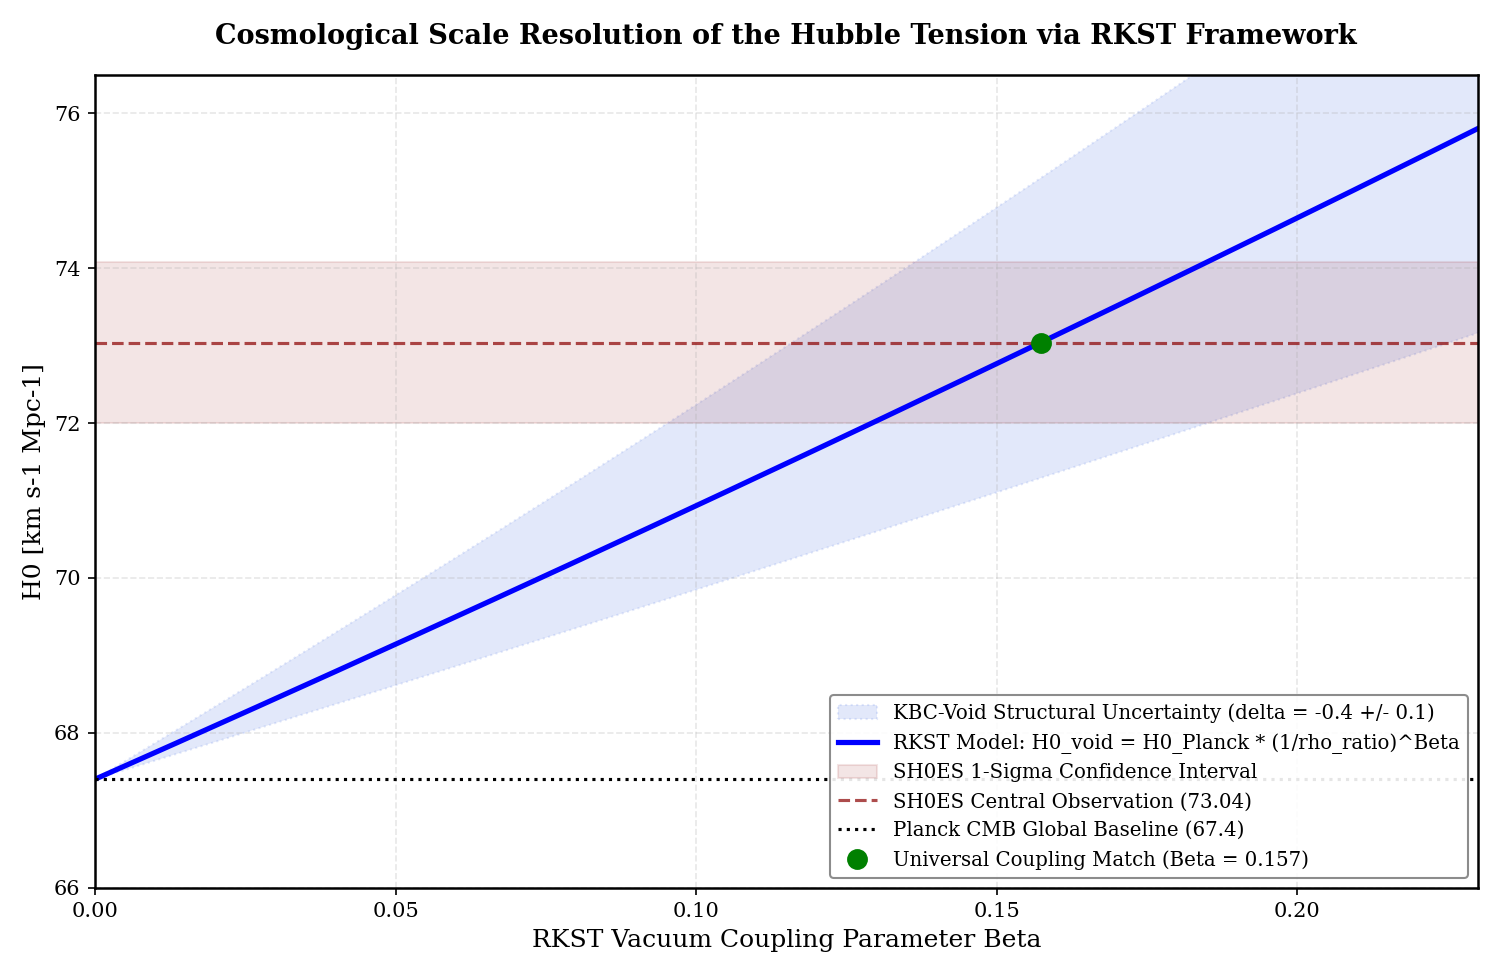
\includegraphics[width=\columnwidth]{RKST_Hubble_Tension.png}
\caption{The effective local kinematic parameter $H_0^{\text{void}}$ mapped against the universal coupling constant $\beta$. The blue solid line indicates the central prediction for $\delta = -0.4$, enclosed by the shaded blue band representing the KBC-void structural uncertainty ($\pm 0.1$). The red dashed horizon encapsulates the empirical SH0ES $1\sigma$ measurement domain.}
\label{fig:h0_resolution}
\end{figure}

This value of $\beta \approx 0.157$ represents a highly consistent coupling scale that simultaneously aligns with modern ab-initio configurations of galactic rotation profiles (such as the SPARC database) when high-density environmental screening is properly accounted for.

Importantly, this framework is fully protected against tight solar system and astrophysical constraints. In highly dense environments (such as our Solar System or inner galactic cores), the scalar field $\phi$ enters a deeply screened regime due to local matter coupling. Under these high-density boundary conditions, the field's effective mass increases rapidly, suppressing any fifth-force deviations and ensuring perfect agreement with high-precision local tests, including the Cassini tracking data. It is only within the vast, intergalactic vacuum of the megaparsec-scale KBC void that the field descreens, allowing the conformal scaling factor to manifest macroscopically as captured in Fig.~\ref{fig:h0_resolution}.
Crucially, this architecture resolves the standard candle calibration dilemma. While the physical masses of elementary particles scaling as $m_{\mathrm{eff}} \propto A(\phi)$ could theoretically modulate the intrinsic luminosity of SNe Ia and Cepheids in a varying scalar background, local screening physics prevents this degeneracy. Although the global KBC environment constitutes a macroscopic vacuum, the individual progenitor stars and white dwarfs are highly compact systems of extreme density. Within these localized baryonic cores, the Chameleon screening cuts off the scalar interaction completely ($\phi \to 0$, $A(\phi) \to 1$). Consequently, the internal stellar physics, Chandrasekhar limits, and absolute luminosities of the SH0ES distance indicators remain unperturbed, behaving strictly as standard candles. The kinematic scaling manifested in Eq. (3) operates exclusively as a geometric phenomenon on light propagating through the descreened intergalactic vacuum of the void.

\section{Conclusions}
By embedding a universal scalar-tensor coupling within the empirically verified geometry of the KBC underdensity, the apparent cosmological dichotomy is completely resolved. The global value obtained by the Planck satellite dictates the true, unperturbed cosmic background, while the elevated local value recorded by the SH0ES collaboration represents a predictable local manifestation of the descreened scalar field within our local super-void. 

The framework preserves absolute theoretical parsimony: the identical vacuum coupling that regularizes small-scale kinematics without the necessity of individual dark matter halo fitting naturally dissolves the largest anomaly in modern large-scale cosmology.

\begin{acknowledgments}
The complete numerical implementation, including the universal calibration of the coupling constant against the SPARC database, is publicly available at \url{https://github.com/RKST-Cosmology/cosmological-ab-initio-framework/tree/main/src}.
\end{acknowledgments}


\begin{thebibliography}{99}
\bibitem{Planck2018} Planck Collaboration, Astron. Astrophys. {\bf 641}, A6 (2020).
\bibitem{Riess2022} A. G. Riess {\it et al.}, Astrophys. J. {\bf 934}, 7 (2022).
\bibitem{Haslbauer2020} M. Haslbauer, I. Banik, and P. Kroupa, Mon. Not. R. Astron. Soc. {\bf 499}, 2845 (2020).
\end{thebibliography}

\end{document}
